% !TEX program = xelatex
\documentclass[12pt,a4paper]{report}

% ── Fonts ────────────────────────────────────────────────────────────────────
\usepackage{fontspec}
% Template fonts are Times New Roman / Arial; fall back to metric-compatible
% Liberation, then to TeX Gyre (bundled with TeX Live) where unavailable.
\IfFontExistsTF{Times New Roman}{\setmainfont{Times New Roman}}{%
  \IfFontExistsTF{Liberation Serif}{\setmainfont{Liberation Serif}}%
    {\setmainfont{TeX Gyre Termes}}}
\IfFontExistsTF{Arial}{\setsansfont{Arial}}{%
  \IfFontExistsTF{Liberation Sans}{\setsansfont{Liberation Sans}}%
    {\setsansfont{TeX Gyre Heros}}}

% ── Page geometry ─────────────────────────────────────────────────────────────
% Left 4 cm, others 2 cm  (Oulu IPS template)
\usepackage[
  a4paper,
  left=4cm,
  right=2cm,
  top=2cm,
  bottom=2cm,
  includeheadfoot,
  headheight=15pt
]{geometry}

% ── Line spacing ──────────────────────────────────────────────────────────────
\usepackage{setspace}
\singlespacing

% ── Headers / footers ─────────────────────────────────────────────────────────
\usepackage{fancyhdr}
\pagestyle{fancy}
\fancyhf{}
\fancyhead[R]{\thepage}
\renewcommand{\headrulewidth}{0pt}
% Chapter opening pages use the "plain" style; give it the same top-right number.
\fancypagestyle{plain}{%
  \fancyhf{}%
  \fancyhead[R]{\thepage}%
  \renewcommand{\headrulewidth}{0pt}%
}

% ── Chapter / section heading fonts  ─────────────────────────────────────────
\usepackage{titlesec}

% Chapter heading: Arial 18pt bold, no "Chapter N" prefix
\titleformat{\chapter}[block]
  {\sffamily\fontsize{18}{22}\bfseries}
  {\thechapter.}{0.5em}{}
\titlespacing*{\chapter}{0pt}{0pt}{12pt}

% Section heading: Arial 14pt bold
\titleformat{\section}[block]
  {\sffamily\fontsize{14}{18}\bfseries}
  {\thesection}{0.5em}{}
\titlespacing*{\section}{0pt}{18pt}{6pt}

% Subsection heading: Arial 14pt (not bold, matching template)
\titleformat{\subsection}[block]
  {\sffamily\fontsize{14}{18}\normalfont}
  {\thesubsection}{0.5em}{}
\titlespacing*{\subsection}{0pt}{12pt}{4pt}

% Unnumbered chapter (Abstract, Foreword, etc.) — same style, no number
\newcommand{\unnumberedchapter}[1]{%
  \chapter*{#1}%
  \addcontentsline{toc}{chapter}{#1}%
}

% ── Paragraph spacing ─────────────────────────────────────────────────────────
\setlength{\parindent}{0pt}
\setlength{\parskip}{10pt}

% ── Text alignment ────────────────────────────────────────────────────────────
\usepackage{ragged2e}
\justifying
% No words split across lines: no hyphenation, and no line breaks at explicit
% hyphens or em dashes (---). The extra inter-word stretch below lets justified
% lines absorb the words that can no longer be split.
\hyphenpenalty=10000
\exhyphenpenalty=10000
\setlength{\emergencystretch}{3em}

% ── Tables ────────────────────────────────────────────────────────────────────
\usepackage{booktabs}
\usepackage{tabularx}
% Table text is left-aligned: justified narrow cells stretch badly without hyphenation.
\renewcommand{\tabularxcolumn}[1]{>{\raggedright\arraybackslash}p{#1}}
\usepackage{array}
\usepackage{longtable}
% Figures and tables never float past the start of the next section.
\usepackage[section]{placeins}
% Pages holding only figures/tables start at the top instead of centring them.
\makeatletter
\setlength{\@fptop}{0pt}
\setlength{\@fpsep}{12pt}
\makeatother
\usepackage{makecell}

% Table caption: Arial 10pt bold, above table
\usepackage{caption}
\captionsetup[table]{
  font={sf,small,bf},
  labelsep=space,
  justification=raggedright,
  singlelinecheck=false,
  position=above
}
\captionsetup[figure]{
  font={sf,small,bf},
  labelsep=period,
  justification=centering,
  position=below
}

% ── Graphics ──────────────────────────────────────────────────────────────────
\usepackage{graphicx}
\usepackage{tikz}
\usetikzlibrary{positioning, arrows.meta, fit, calc, shapes.geometric}

% ── Hyperlinks ────────────────────────────────────────────────────────────────
\usepackage[hidelinks]{hyperref}
\usepackage{xurl}                    % allow long URLs/DOIs to break across lines

% ── Math ─────────────────────────────────────────────────────────────────────
\usepackage{amsmath}
\usepackage{amssymb}

% ── Misc ──────────────────────────────────────────────────────────────────────
\usepackage{enumitem}
\usepackage{microtype}
\usepackage{eurosym}
\usepackage{xcolor}

% ── Hanging references ────────────────────────────────────────────────────────
\usepackage{hanging}

% ══════════════════════════════════════════════════════════════════════════════
\begin{document}

% ── COVER PAGE ──────────────────────────────────────────────────────────────
\newgeometry{left=2cm, right=2cm, top=2cm, bottom=2cm, nohead, nofoot}
\begin{titlepage}
\setlength{\parskip}{0pt}
\centering
\vspace*{3cm}

\includegraphics[width=3.76cm, keepaspectratio]{attachments/uni_logo.jpeg}\par
\vspace{3.53cm}
{\sffamily\fontsize{20}{24}\bfseries
Design of a Multi-Agent Home Energy Gateway: Interpreting Household
Plans and Configuring an Optimiser\par}
\vfill
{\raggedright\leftskip=10.16cm\rmfamily\normalsize
University of Oulu\\
Information Processing Science\\
Master's Thesis\\
Hoan Le\\
2026\par}
\end{titlepage}
\restoregeometry

\pagenumbering{arabic}
\setcounter{page}{1}

% ── ABSTRACT ────────────────────────────────────────────────────────────────
\unnumberedchapter{Abstract}

In process.

\vspace{12pt}
{\sffamily\itshape Keywords}

\vspace{4pt}
home energy management, energy gateway, multi-agent system, ReAct, large
language model, model predictive control, plan interpretation, Design
Science Research

\vspace{12pt}
{\sffamily\itshape Supervisor}

\vspace{4pt}
Yueqiang Xu, PhD, Docent, Adjunct Professor

\vspace{4pt}
Paula Alavesa, PhD

% ── FOREWORD ────────────────────────────────────────────────────────────────
\unnumberedchapter{Foreword}

In process.

% ── ABBREVIATIONS ───────────────────────────────────────────────────────────
\unnumberedchapter{Abbreviations}

\begin{description}[leftmargin=5cm, style=nextline, font=\normalfont\bfseries, before=\raggedright]
\item[BDEW] German Association of Energy and Water Industries (Bundesverband der Energie- und Wasserwirtschaft)
\item[COP] Coefficient of Performance (of a heat pump)
\item[DSR] Design Science Research
\item[DWD] German Weather Service (Deutscher Wetterdienst)
\item[EEG] Renewable Energy Sources Act (Erneuerbare-Energien-Gesetz)
\item[EMC] Energy Management Controller
\item[EMHASS] Energy Management for Home Assistant
\item[EnWG] Energy Industry Act (Energiewirtschaftsgesetz)
\item[EV] Electric Vehicle
\item[HEMS] Home Energy Management System
\item[LLM] Large Language Model
\item[LP] Linear Programming
\item[MILP] Mixed-Integer Linear Programming
\item[MPC] Model Predictive Control
\item[OCPP] Open Charge Point Protocol
\item[OPSD] Open Power System Data
\item[PV] Photovoltaic (rooftop solar panels)
\item[ReAct] Reasoning and Acting
\item[SLR] Systematic Literature Review
\item[SoC] State of Charge (of a battery)
\item[SQ] Sub-question
\end{description}

% ── DECLARATION OF GENERATIVE AI ─────────────────────────────────────────────
\unnumberedchapter{Declaration of Generative AI in the Thesis}

In process.

% ── TABLE OF CONTENTS ───────────────────────────────────────────────────────
\tableofcontents

% ════════════════════════════════════════════════════════════════════════════
\chapter{Introduction}
\label{ch:intro}

\section{Background and problem}
\label{sec:problem}

A home energy gateway is the device in the meter cabinet or on the home
network that reads the smart meter and controls the home's energy
assets: the rooftop photovoltaic (PV) system and its inverter, a home
battery, a heat pump, an electric vehicle (EV) charger and smart
appliances. Its task is to decide, every few minutes, when each asset
draws, stores or exports power, so that the household pays less, uses
more of its own solar power and stays within the limits set by the grid
operator. Figure~\ref{fig:homesystem} shows such a system.

\begin{figure}[htbp]
\centering
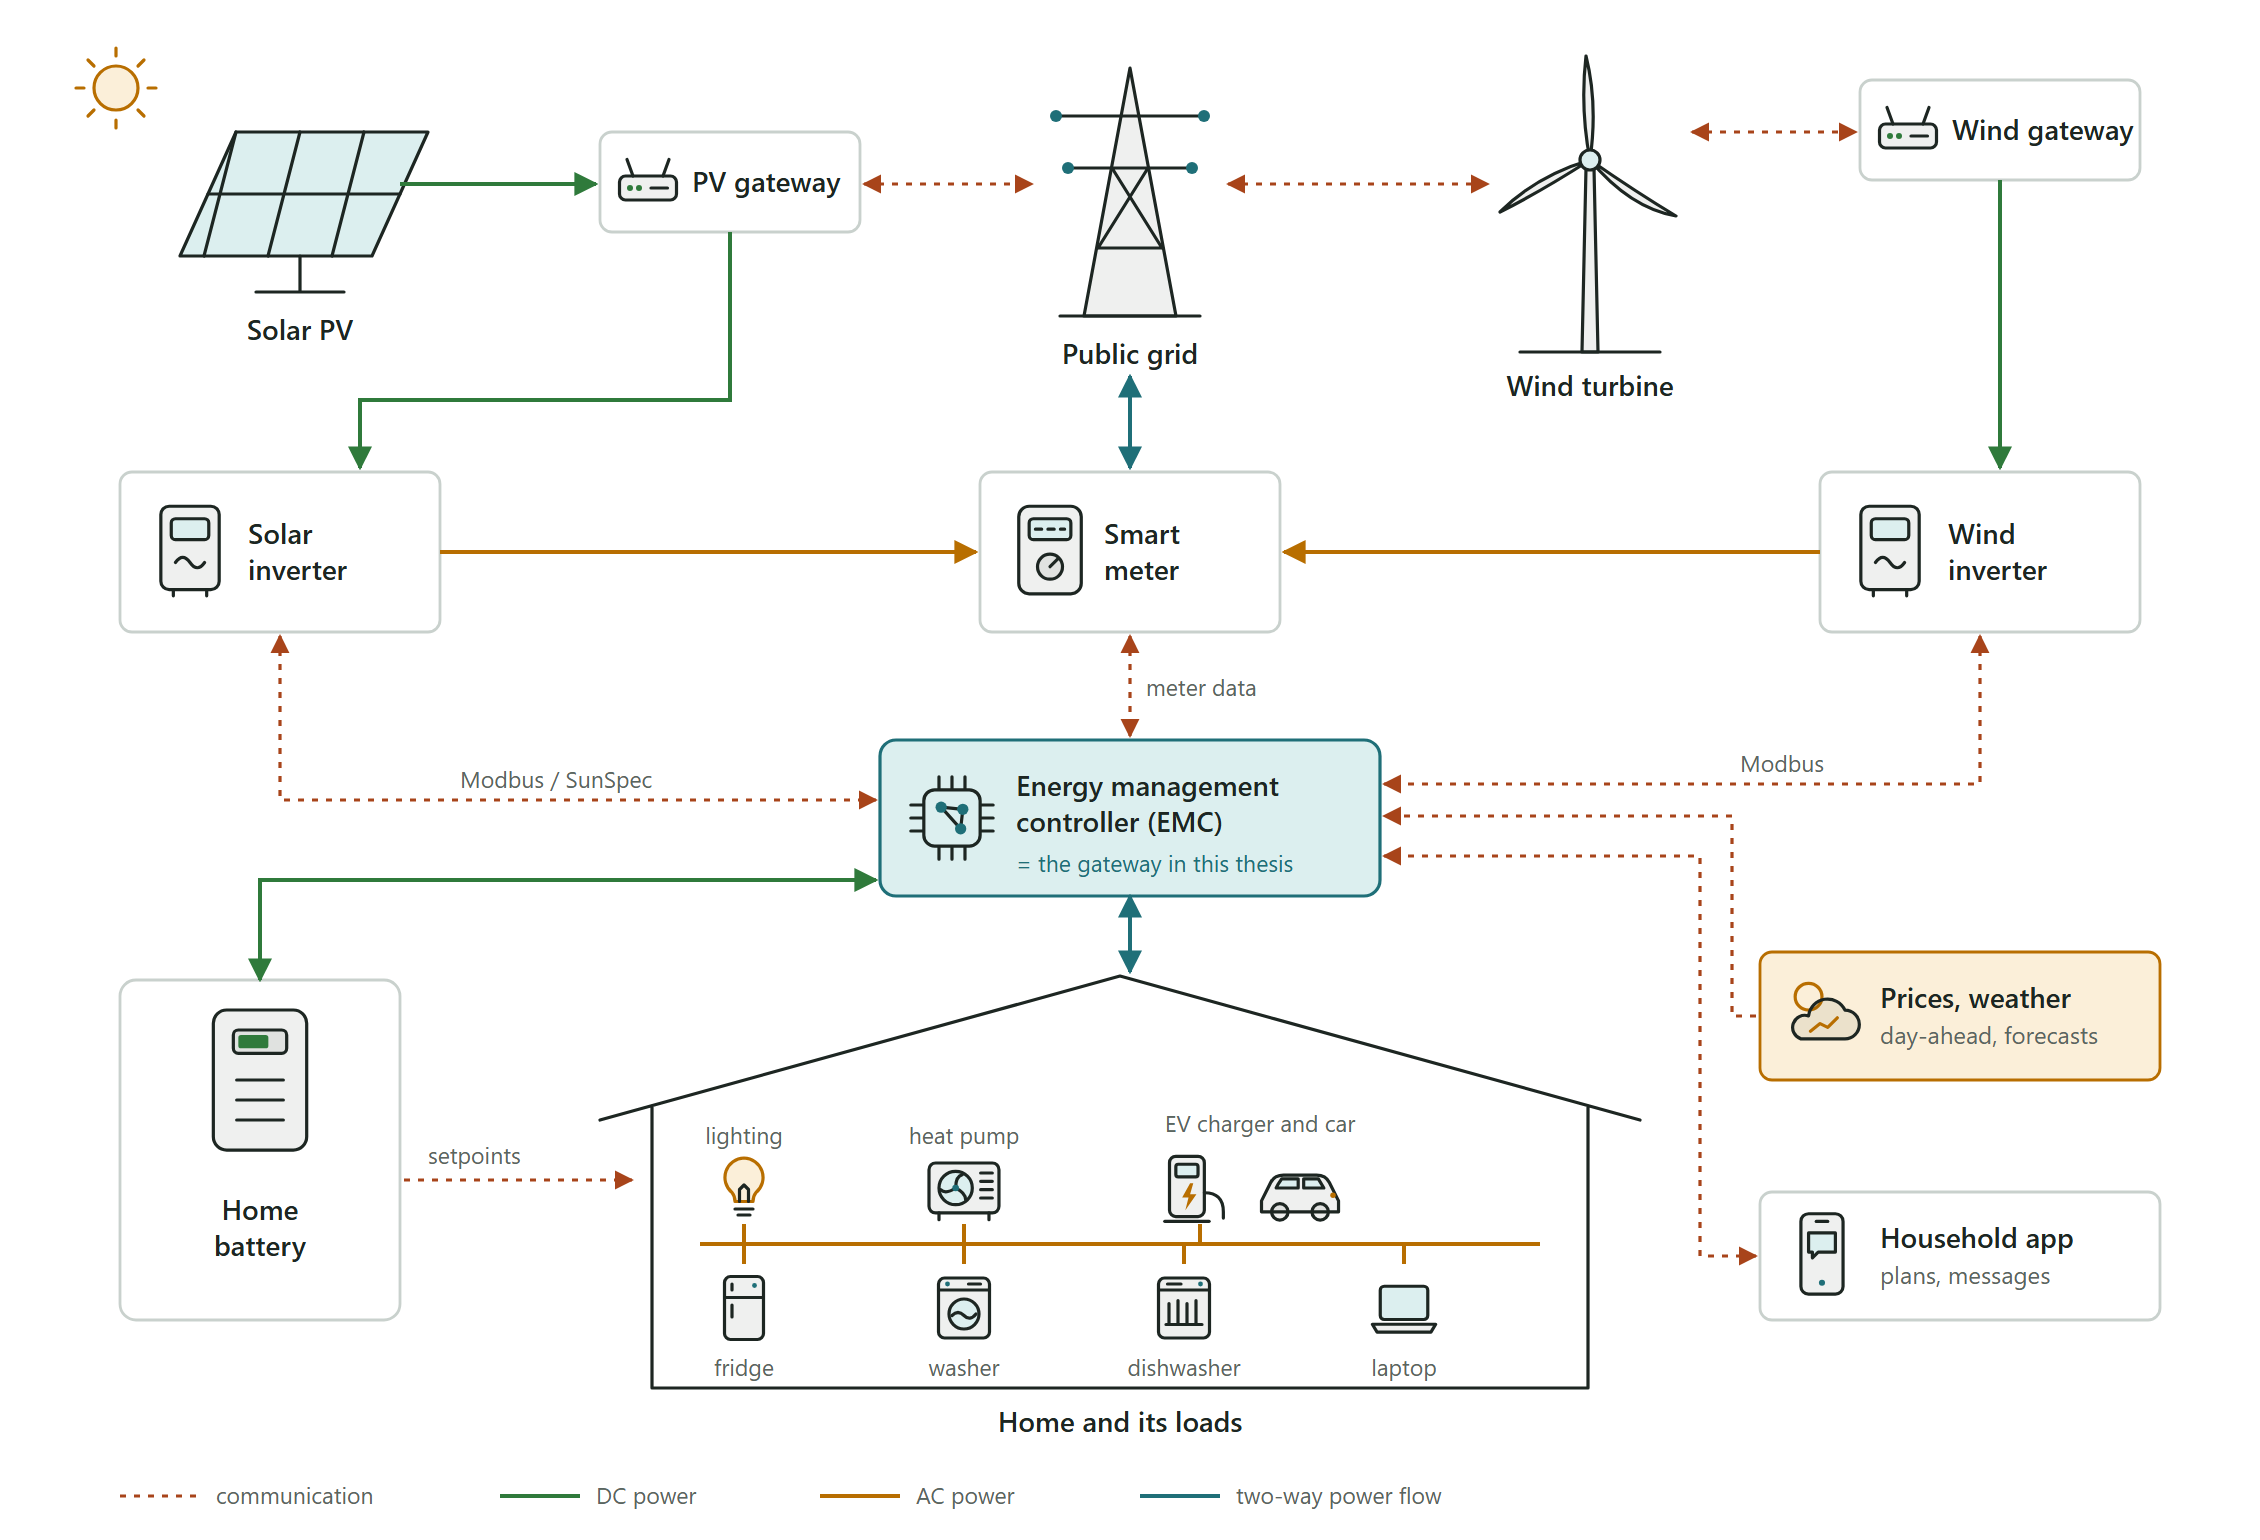
\includegraphics[width=\textwidth]{attachments/gateway/home_energy_system.png}
\caption{A home energy system and its controller. The energy management
controller (EMC) is the gateway studied in this thesis.}
\label{fig:homesystem}
\end{figure}

Four problems limit what today's gateways achieve.

\textit{Devices do not share one language.} Inverters, batteries,
chargers and heat pumps from different makers communicate in different
ways, many only through their manufacturer's cloud, and standards such
as Matter and OpenADR are adopted slowly (Energy Systems Catapult, 2026).

\textit{Several controllers act on one device.} An EV charger can
receive commands from the car's app, the charger's app, a smart-charging
service, a flexibility service and the energy supplier
(Energy Systems Catapult, 2026).

\textit{The grid operator sets limits.} In Germany, heat pumps and
wallboxes above 4.2\,kW installed since 2024 must accept power
reductions from the grid operator through the smart meter gateway and a
control box (§14a of the Energy Industry Act, EnWG), so the household's
plan has to fit inside an external limit (evcc, n.d.).

\textit{Planning by fixed rules leaves savings unused, and an optimiser
needs an expert.} Typical gateways follow rules such as ``charge the car
from PV surplus''. Model predictive control (MPC), which plans ahead
with price and weather forecasts, lowered the energy cost of a PV and
battery home by 13.5\,\% against a rule-based strategy
(Seal et al., 2019), and stochastic MPC performed best under realistic
forecast errors (Blonsky et al., 2022). An MPC, however, needs exact
parameters: when the car leaves and how full it must be, the comfort
band of each period, the battery reserve and how far to trust the PV
forecast. Households do not think in these parameters, settings become
outdated when routines, seasons or tariffs change, and complicated
systems slow adoption (Tuomela et al., 2021).

Language-model agents can bridge the gap between what a household says
and what an optimiser needs. Recent work turns plain-language
preferences into optimisation constraints
(Sanguinetti et al., 2025; Michelon et al., 2025) or lets ReAct agents schedule
appliances directly (El Makroum et al., 2026; Jonah et al., 2026). Direct
schedulers come close to the optimum, but they also produced invented
schedules and misstated deadlines, and their authors recommend a
deterministic validator before any device is switched
(Jonah et al., 2026). The author's earlier thesis reached the same
conclusion for appliance scheduling: reliability and savings came from
the solver and the deterministic checks, not from the language model or
the number of agents (Le, 2026).

This thesis therefore gives the agents the work an optimiser cannot do:
interpreting the household's plans and changes, configuring the
optimiser from the house's own history, reacting to events and
explaining the plan. The optimiser computes the schedule, and a
deterministic checker and control layer switch the devices.

\section{Research questions}
\label{sec:rq}

The main research question is:

\textbf{RQ:} How can a language-model agent let a home energy gateway
work from the household's plain-language plans without expert
configuration, by interpreting the plans and configuring and explaining
an optimiser, while keeping control reliable?

Four sub-questions (SQ) divide it:

\begin{description}[leftmargin=1.4cm, style=sameline, font=\normalfont\bfseries]
\item[SQ1] \textit{Interpretation.} How accurately does the agent turn
plain-language plans and their changes into constraints and a
commit-or-ask decision, and how often are the household's requirements
then met?
\item[SQ2] \textit{Configuration.} Can the agent configure the MPC from
the house's history close to an expert-tuned MPC, and better than a
deterministic auto-tuner that sees the same history?
\item[SQ3] \textit{Reliability and cost.} How often do the checker and
the fallback intervene, what does the agent cost locally and in the
cloud, and does splitting the work into four agents help compared with
one or two?
\item[SQ4] \textit{Conditions.} Under which weather, price patterns,
household loads and plan types does interpretation or configuration
fail?
\end{description}

The thesis does not measure usability with users. Its claim is that the
gateway works without expert configuration from plans written by people
other than the author; a usability study is left for future work.

\section{Research approach and scope}

The thesis follows Design Science Research (DSR)
(Hevner et al., 2004; Peffers et al., 2007): an artifact is designed, built,
demonstrated and evaluated, with design iterations on an exploratory set
and a registered confirmation on a held-out set
(Chapter~\ref{ch:method}). The evaluation is limited to households: one
home with PV, a battery, a heat pump and an EV charger is simulated
with measured data, real weather and real prices
(Section~\ref{sec:data}). Transferability to industrial energy
management is discussed in Section~\ref{sec:industry}.

\section{Structure of the thesis}

Chapter~\ref{ch:lit} reviews related work. Chapter~\ref{ch:method}
describes the research method, the data and the evaluation design.
Chapter~\ref{ch:design} presents the artifact. Chapter~\ref{ch:results}
reports the exploratory pilots; the registered evaluation is in process.
Chapters~\ref{ch:discussion} and~\ref{ch:conclusions} discuss and
conclude.

% ════════════════════════════════════════════════════════════════════════════
\chapter{Literature Review}
\label{ch:lit}

The systematic literature review (SLR) defined in
Section~\ref{sec:slr} is in process. This chapter summarises the
studies already read, grouped by the parts of the design they inform.

\section{Home energy management and optimisation}

Home energy management systems (HEMS) schedule household loads, storage
and generation against prices and comfort requirements; reviews classify
the methods into rule-based control, mathematical optimisation, MPC and
heuristics (Beaudin \& Zareipour, 2015). MPC re-solves an optimisation over a
receding horizon with updated forecasts. Against a rule-based strategy,
a centralised MPC lowered the energy cost of a PV and battery home by
13.5\,\% (Seal et al., 2019). Under realistic uncertainty in weather,
occupant behaviour and building parameters, stochastic MPC performed
better than deterministic MPC and heuristics (Blonsky et al., 2022).
Open-source tools bring optimisation into homes: EMHASS solves a
day-ahead linear programme for Home Assistant installations
(EMHASS contributors, 2026). The gap between such tools and households is
configuration: the optimiser must be told the household's requirements
and parameters, and the systems that require it are perceived as too
complicated (Tuomela et al., 2021).

\section{Language-model agents in home energy management}

Language models are used in home energy management in two roles.
\textit{As an interface}, they translate what a user says into the
inputs of an optimiser. Michelon et al. (2025) combine ReAct with
few-shot prompting to extract the parameters a HEMS needs and report an
average parameter retrieval accuracy of 88\,\%.
Sanguinetti et al. (2025) map natural-language appliance preferences
onto optimisation constraints for household batteries in an energy
community. \textit{As a scheduler}, agents plan loads themselves.
El Makroum et al. (2026) coordinate several appliances with a ReAct
orchestrator and specialist agents; Jonah et al. (2026) compare tool-calling agents on half-hourly
prices and find that native function calling outperforms text-parsed
actions and that low cost does not guarantee feasible behaviour.
Raghavan and Giridhar (2025) pair a zero-shot agent with MPC, and multi-agent
designs for home and building energy management are appearing
(Jung, 2026; Yang et al., 2025; Liu et al., 2025). Zhang and Chen (2024) use a
language model to make building control interpretable. The author's
earlier thesis evaluated a hierarchical ReAct pipeline for appliance
recommendations and found that the solver and the deterministic checks,
not the agents, produced the savings and the validity (Le, 2026).

\section{From natural language to optimisation models}

Outside the energy domain, the NL4Opt competition defined the task of
turning a word problem into an optimisation model
(Ramamonjison et al., 2023). OptiMUS formulates and solves
mixed-integer linear programmes from natural-language descriptions with
a language-model agent that writes and debugs solver code
(AhmadiTeshnizi et al., 2024), and Chain-of-Experts divides the
formulation among cooperating expert agents (Xiao et al., 2024). These
works generate the whole model; this thesis keeps a fixed, verified
model and lets the agent set only its constraints and parameters.

\section{Safety envelopes for unverified controllers}

The Simplex architecture runs a high-performance but unverified
controller inside an envelope of a simple, verified controller that
takes over when the unverified one would leave the safe region
(Sha, 2001). The deterministic checker and control layer of the
gateway play the role of the verified envelope around the language-model
agents.

\section{Research gap}

The studies above either let the language model produce schedules,
which needs a validator, or extract parameters for a single request.
None was found that (1) lets agents configure an MPC from a house's own
history and compares them with a deterministic auto-tuner, (2) handles
plans and changes during the day for PV, battery, heat pump and EV
together, checked before execution, and (3) evaluates against a tuned
rather than a default optimiser. Whether this gap holds is part of the
SLR, which is in process.

% ════════════════════════════════════════════════════════════════════════════
\chapter{Research Methodology}
\label{ch:method}

\section{Design Science Research}

The artifact is one home energy gateway with an agent layer of four
agents and a deterministic harness (Chapter~\ref{ch:design}). Following
Peffers et al. (2007), the work runs in three cycles:

\begin{enumerate}[nosep]
\item \textit{Cycle 1 (done):} exploratory prototypes: a digital twin
of the house, a gateway pilot with planning agents, a
plan-interpretation pilot and a Configurator pilot
(Chapter~\ref{ch:results}).
\item \textit{Cycle 2 (in process):} the tools and agents of the
four-agent design, iterated on an exploratory set of house-days.
\item \textit{Cycle 3 (in process):} a registered evaluation on a
held-out set and a year simulation.
\end{enumerate}

\section{Systematic literature review}
\label{sec:slr}

The review follows Kitchenham and Charters (2007) with backward and forward
snowballing (Wohlin, 2014). Scopus and Web of Science are
searched for peer-reviewed work and arXiv and Google Scholar for 2025
and 2026 preprints. The search string combines three blocks: home
energy management terms (``home energy management'', ``residential
demand response'', ``home energy gateway''), language-model terms
(``large language model*'', ``LLM-based'', ``agentic'', ``ReAct'') and,
in a second run, optimisation terms (``model predictive control'',
``MILP'', ``scheduling''). Included are studies from 2022 to 2026 on
behind-the-meter assets in which a language model generates
constraints, tunes parameters, schedules loads or controls devices, and
which evaluate the system. The search results are in process.

\section{Data}
\label{sec:data}

Table~\ref{tab:data} lists the data. The main house is site
\texttt{DE\_KN\_residential4} of the OPSD Household data package
(Open Power System Data, 2020): measured 15-minute energy data from homes in
Konstanz, Germany, with PV generation, grid import and export, a heat
pump, an EV and appliances. In 2016 the house's PV produced about
11.0\,MWh, the heat pump used 2.6\,MWh and the EV 1.0\,MWh. Weather,
prices and heat pump efficiency come from the same place and dates.

\begin{table}[!ht]
\caption{Data used in the evaluation.}
\label{tab:data}
\small
\begin{tabularx}{\textwidth}{@{}p{3.3cm}Xp{3.0cm}@{}}
\toprule
Data & Content and source & Use \\
\midrule
OPSD Household data & 15-minute PV, grid, heat pump, EV and appliance data of homes in Konstanz, 2014--2019 (Open Power System Data, 2020) & main house; more houses for SQ2 \\
DWD station 02712 & hourly air temperature and global radiation, Konstanz (Deutscher Wetterdienst, n.d.) & weather classes, forecasts \\
Day-ahead prices & German spot prices, 2015--2019 (Fraunhofer ISE, n.d.) & import and export price \\
BDEW price analysis & 2016 household price components, 28.80\,ct/kWh (BDEW, 2023) & dynamic tariff \\
EEG feed-in tariff & 12.31\,ct/kWh for rooftop PV up to 10\,kWp (Bundesnetzagentur, n.d.) & export price \\
When2Heat & heat pump COP by hour (Ruhnau et al., 2019; Ruhnau \& Muessel, 2023) & heat demand from heat pump electricity \\
Norwegian EV sessions & 35,377 residential charging sessions (Sørensen et al., 2024) & optional: departure times \\
Plan benchmark & plain-language plans with answer keys (pilot set in Appendix~\ref{app:plans}) & SQ1 ground truth \\
\bottomrule
\end{tabularx}
\end{table}

The import price is a counterfactual dynamic tariff built from the 2016
components: (spot price + supplier margin + 17.94\,ct/kWh of fees and
levies) $\times$ 1.19 VAT. A PV model fitted to DWD global radiation
reproduces the house's PV with a correlation of 0.96 hourly and 0.98
daily.

\section{Evaluation design}

\textit{Benchmark.} The unit is a house-day of 96 fifteen-minute slots
with a plain-language plan and, where the design calls for it, a change
during the day. Factors are the plan type (structured, plain language,
plain language with a change, ambiguous, conflicting or infeasible),
weather, price pattern, load and house. Plans for the held-out set are
written by three to five people other than the author, keyed before
any run and checked by a second person.

\textit{Systems.} All systems use the same house-days, forecasts, plans
and control layer: the recorded operation; rules; EMHASS; default MPC;
an expert-tuned MPC (settings chosen once on exploratory weeks and
frozen); a deterministic auto-tuner (weekly grid search over past weeks);
a language model without tools; the four-agent gateway with a cloud
and a local model; ablations with one and two agents; and perfect
foresight as the upper bound.

\textit{Metrics.} Constraint precision and recall against the answer
key, clarification F1 and decision accuracy (SQ1); household
requirements met; adjusted cost, which subtracts the value of battery
charge and stored heat left at midnight; the share of the gap between
rules and perfect foresight that a system closes; rejected plans,
fallbacks and failed calls; tokens, cost, mean and 95th-percentile
latency and energy per event.

\textit{Hypotheses (draft, to be registered).} H1: constraint precision
and recall of at least 0.90 and a clarification F1 of at least 0.85;
H2: household requirements met on at least 95\,\% of feasible
house-days; H3: plain-language plans cost no more than the same plans
given as exact parameters to the tuned MPC, within 5\,\% of the
rules-to-optimum gap; H4a and H4b: the agent-configured MPC closes a
registered share of the gap between default and tuned MPC and is
non-inferior to the auto-tuner; H5: the best local model is within 0.10
of the cloud model's recall; H6: the yearly saving exceeds the gateway's
own cost with cloud inference and with a local inference box. The
analysis uses cluster bootstrap intervals over plans, exact binomial and
paired Wilcoxon tests, and Holm correction within SQ1 and within SQ2.

\textit{Validity.} The main threats and their handling are author-written
plans (other writers, second-person check), tuning on evaluation days
(tuning only on exploratory weeks), a harness that passes H2 by
construction (scoring against the answer key, with grid and battery
limits reported separately as safety checks), mixed data sources (same
place and dates, the dynamic tariff stated as counterfactual) and
simulation only (a field study as future work).

% ════════════════════════════════════════════════════════════════════════════
\chapter{System Design and Implementation}
\label{ch:design}

\section{Requirements}

From the problem (Section~\ref{sec:problem}) follow five requirements:
(R1) the household states its plans in plain language; (R2) the gateway
is configured without an expert; (R3) no language model computes a
schedule or switches a device; (R4) every plan passes a deterministic
check before it takes effect; (R5) the house stays within its limits
when an agent, a model or the network fails.

\section{Architecture}

The gateway has three layers (Figure~\ref{fig:architecture}). The
\textit{agent layer} holds four agents, each started by one kind of
event. The \textit{harness} holds the tools, a tuned MPC that replans
every hour on its own, a checker and a history store. The
\textit{control layer} runs every 15 minutes, holds the planned grid
exchange so that the battery absorbs forecast errors, keeps comfort,
the EV deadline and the battery limits, and falls back to rules. The
harness follows the Simplex pattern (Sha, 2001): the agents are
unverified controllers inside a verified envelope.

\begin{figure}[htbp]
\centering
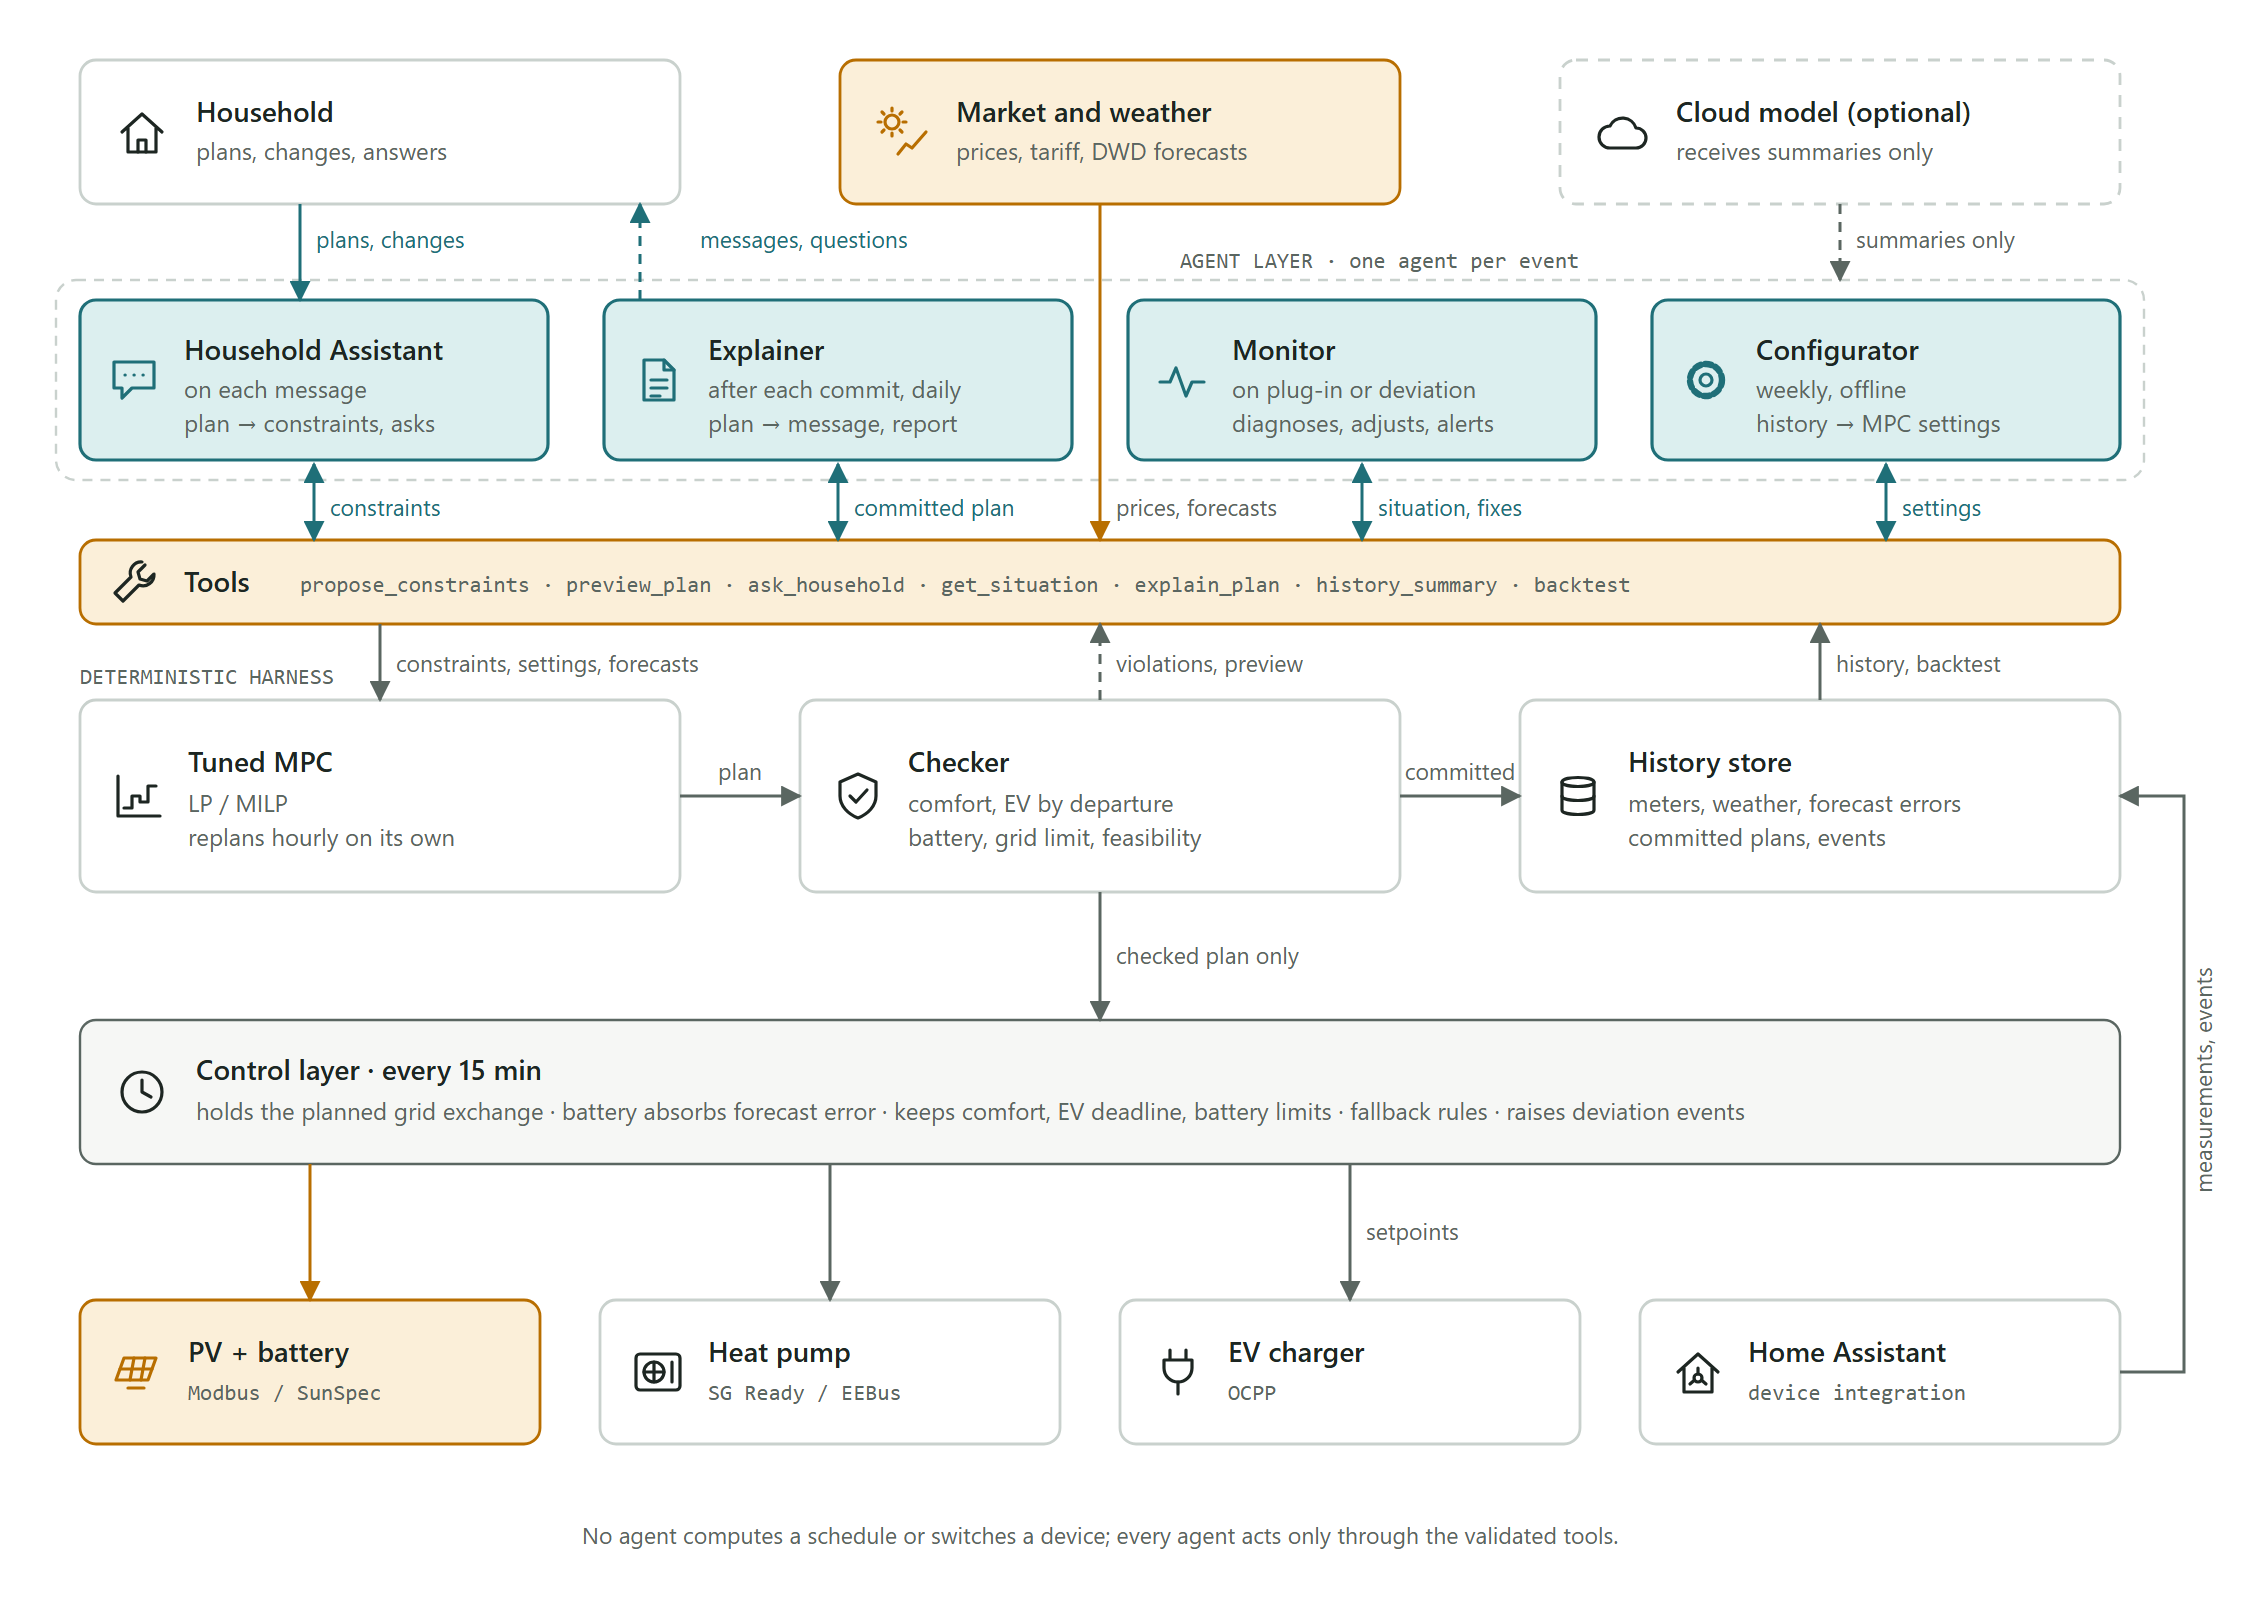
\includegraphics[width=\textwidth]{attachments/gateway/architecture.png}
\caption{Architecture of the gateway: four agents act only through
validated tools; the tuned MPC plans and the checker passes only valid
plans to the control layer.}
\label{fig:architecture}
\end{figure}

\section{Four agents, one per event}

Table~\ref{tab:agents} lists the agents. The harness routes each event
to one agent by its type; no agent calls another, and the agents share
state only through the harness. Splitting by event keeps each prompt
small and lets each output be checked on its own. The earlier thesis
found that splitting \textit{one} task between agents added cost
without reliability (Le, 2026); here the agents do different
tasks at different times, and the agent count is tested as part of SQ3.

\begin{table}[htbp]
\caption{The four agents.}
\label{tab:agents}
\small
\begin{tabularx}{\textwidth}{@{}p{2.8cm}p{3.2cm}X@{}}
\toprule
Agent & Started by & Job \\
\midrule
Household Assistant & a message from the household & turns the plan or change into constraints, previews them, commits or asks \\
Explainer & each commit; once a day & writes the message and the daily report from the committed plan's figures \\
Monitor & an EV plug-in; a deviation raised by the control layer & finds the cause, adjusts constraints within what the household asked, or alerts \\
Configurator & once a week & proposes MPC settings from the house's history and backtests them \\
\bottomrule
\end{tabularx}
\end{table}

Every agent follows the same pattern (Figure~\ref{fig:flow}): it uses
its tools in a short loop and ends at a deterministic gate. The checker
gates the Assistant and the Monitor, a figure check gates the Explainer,
and a backtest gates the Configurator. Only a passed gate changes the
plan, the message or the settings.

\begin{figure}[htbp]
\centering
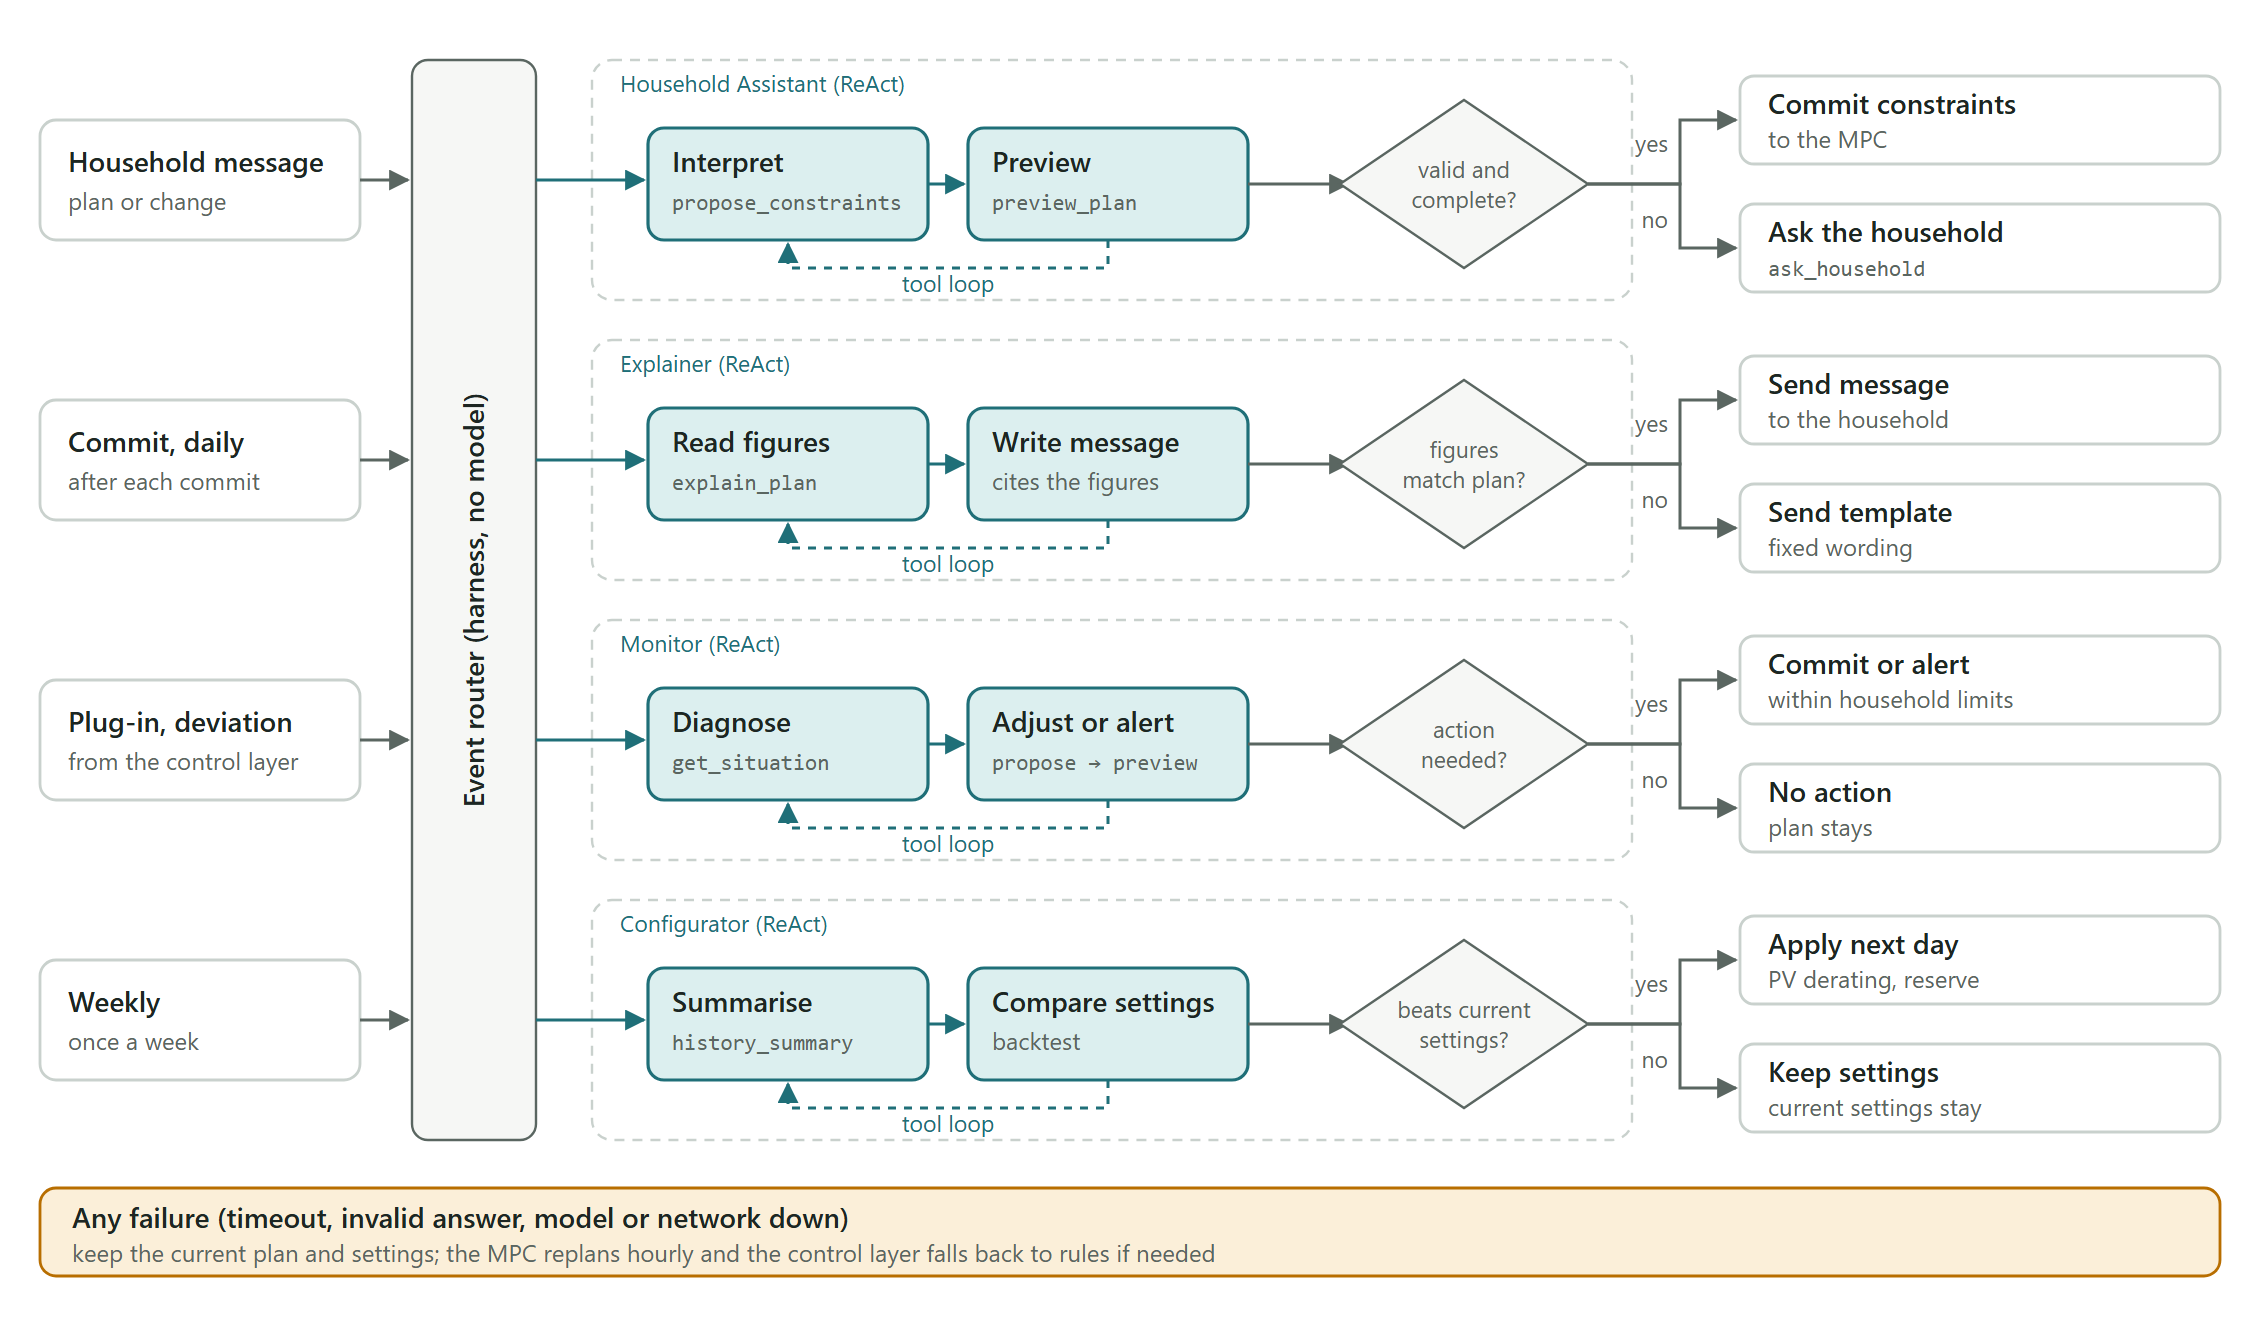
\includegraphics[width=\textwidth]{attachments/gateway/agent_flow.png}
\caption{How each agent decides.}
\label{fig:flow}
\end{figure}

\section{Tools}

The Assistant reads the plan (\texttt{read\_plan}), the situation
(\texttt{get\_situation}) and the forecast (\texttt{get\_forecast}),
proposes constraints (\texttt{propose\_constraints}: EV energy and
departure, comfort bands by time, away periods and appliance windows,
validated against ranges), previews the plan with the MPC and the
checker (\texttt{preview\_plan}), and asks the household only for
ambiguity, conflict or infeasibility (\texttt{ask\_household}). The
Explainer words pre-computed figures (\texttt{explain\_plan}); every
figure it cites is compared with the plan. The Configurator reads
weekly statistics (\texttt{history\_summary}) and compares candidate
settings on past weeks (\texttt{backtest}). Feasibility, for example
more energy than the charger can deliver before departure, is computed
by the checker, not by the language model. Figure~\ref{fig:day} shows
one day at runtime.

\begin{figure}[htbp]
\centering
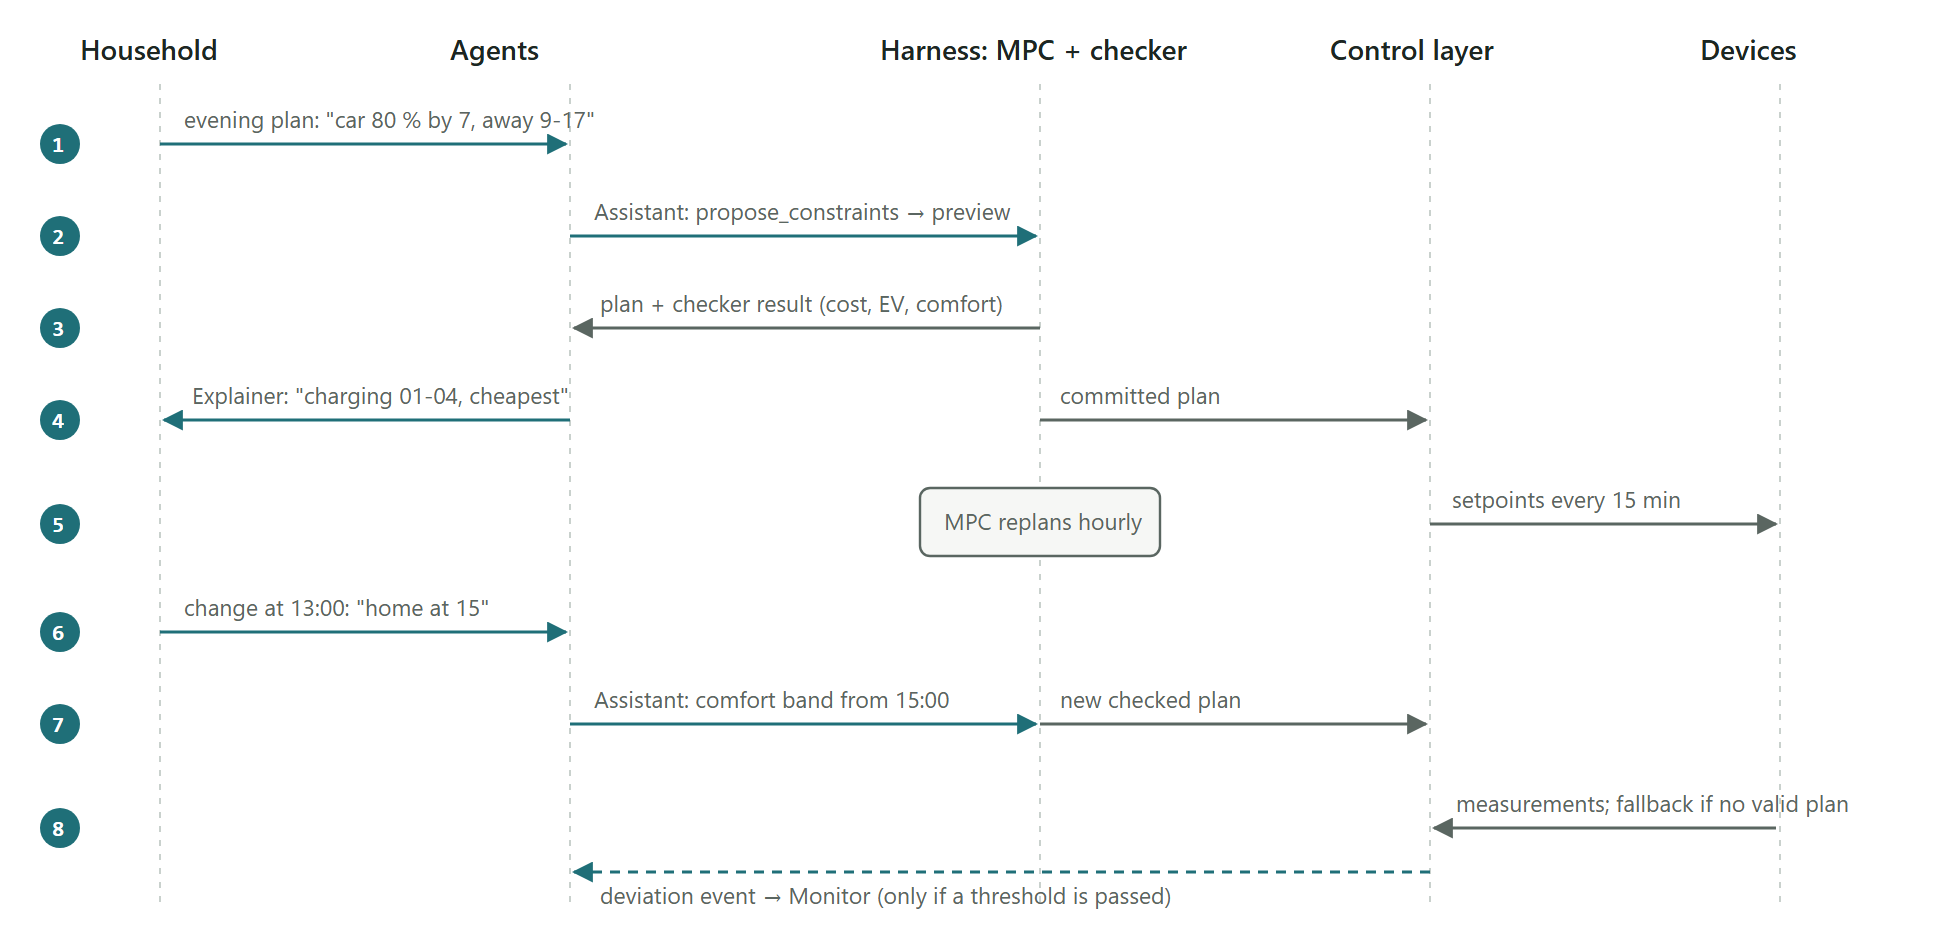
\includegraphics[width=0.9\textwidth]{attachments/gateway/runtime_day.png}
\caption{One day at runtime. Between agent calls the MPC replans every
hour and the control layer runs every 15 minutes without a language
model.}
\label{fig:day}
\end{figure}

\section{Implementation}

The prototypes are written in Python. The digital twin replays the
OPSD house with a virtual 10\,kWh / 5\,kW battery; the MPC is a linear
programme solved with PuLP and CBC from the measured state to midnight,
and energy left at midnight is valued in the same way in the optimiser
and in the score. The agents use LangChain and LangGraph ReAct agents
with structured outputs and a recovery step that returns invalid
answers with the validation errors. Models are GPT-6 Luna through the
OpenAI API and local models through Ollama. The implementation of the
full four-agent design is in process.

% ════════════════════════════════════════════════════════════════════════════
\chapter{Evaluation and Results}
\label{ch:results}

All results in this chapter are exploratory: one house, one run per
configuration and draft answer keys. They guided the design and are not
tests of the hypotheses.

\section{Gateway pilot: agents as planners}
\label{sec:gatewaypilot}

The first pilot let a ReAct agent plan the gateway at four checkpoints a
day (00, 06, 12 and 18\,h and each EV plug-in), with an MPC tool whose
settings it chose. Twelve days of 2016, one per month, were run with
German prices and weather-driven forecasts. Table~\ref{tab:gatewaypilot}
shows the share of the cost gap between rules and perfect foresight
that each strategy closed.

\begin{table}[htbp]
\caption{Gateway pilot, 12 days of 2016: adjusted cost (negative values
are net income from feed-in) and share of the rules-to-optimum gap
closed.}
\label{tab:gatewaypilot}
\small
\begin{tabularx}{\textwidth}{@{}Xrr@{}}
\toprule
Strategy & Adjusted cost (EUR) & Gap closed \\
\midrule
Rules & $-4.79$ & 0\,\% \\
Day-ahead plan & $-5.50$ & 19\,\% \\
Default MPC at checkpoints & $-5.65$ & 23\,\% \\
Default MPC hourly & $-5.97$ & 31\,\% \\
Agent, GPT-6 Luna & $-6.13$ & 36\,\% \\
Agent, gpt-oss-20b (local) & $-6.25$ & 39\,\% \\
MPC with PV derating 0.9, at checkpoints / hourly & & 46\,\% / 51\,\% \\
Perfect foresight & $-8.54$ & 100\,\% \\
\bottomrule
\end{tabularx}
\end{table}

The agents beat the default MPC because they planned with less of the
PV forecast; one fixed setting did this better. GPT-6 Luna made 63
checks with no errors for USD 0.025 in total; gpt-oss-20b made 63
checks with three malformed calls caught by the fallback and took about
152\,s per day. The derating of 0.9 was chosen on the same 12 days, a
weakness the later pilot exposed (Section~\ref{sec:configpilot}). The
pilot changed the design: the agent no longer plans, the MPC replans
hourly without it, and the control layer holds the planned grid exchange
instead of the planned battery power.

\section{Plan-interpretation pilot}
\label{sec:planpilot}

The second pilot tested SQ1 on 22 edge-case plans for the main house
(Appendix~\ref{app:plans}): six simple plans, five changes during the
day, six ambiguous and five conflicting or infeasible requests, each
bound to a date of 2016 and the car's charge. The model returned the
plan as a structured \texttt{HouseholdPlan} with a commit-or-ask
decision, through function calling with up to two validation retries.
Items matched the answer key within 15 minutes, five percentage points
of EV charge or 1\,kWh.

\begin{table}[htbp]
\caption{Plan-interpretation pilot, 22 plans.}
\label{tab:planpilot}
\small
\begin{tabularx}{\textwidth}{@{}Xrrrrr@{}}
\toprule
Model & Precision & Recall & Clarif.\ F1 & Decision & s per plan \\
\midrule
GPT-6 Luna (cloud) & 1.00 & 1.00 & 0.95 & 0.95 & 2.7 \\
gpt-oss-20b (local) & 0.63 & 0.44 & 0.75 & 0.59 & 116 \\
Qwen3 8B (local) & 0.96 & 1.00 & 0.67 & 0.68 & 71 \\
Gemma 4 E4B (local) & 1.00 & 0.91 & 0.78 & 0.82 & 7.7 \\
Qwen3 30B-A3B (local, CPU) & 1.00 & 0.96 & 0.84 & 0.86 & 150 \\
\bottomrule
\end{tabularx}
\end{table}

GPT-6 Luna made one error: for ``charge the car to 90\,\% before I head
out'' it assumed a departure time and committed instead of asking.
gpt-oss-20b often left numbers such as the EV target out and asked
questions that simple plans did not need. Three newer open-weight models
ran on the same laptop (RTX 4070, 8\,GB), with output capped at 8,000
tokens per call after Qwen3 8B looped in its reasoning phase on one
plan. All three extracted items almost as well as the cloud model; they
differed in when they asked. Qwen3 8B committed on almost half of the plans
that needed a question, Gemma 4 E4B missed most conflicts but answered
in under 8 seconds, and Qwen3 30B-A3B came closest to the cloud model
but had to run on the CPU and took two and a half minutes per plan. The
cloud model is close to the ceiling on these cases, which is why the
held-out plans are written by other people. No local model yet meets
H5 on both accuracy and latency; Gemma 4 E4B and Qwen3 30B-A3B are the
candidates for the exploratory phase.

\section{Configurator pilot}
\label{sec:configpilot}

The third pilot tested the riskiest part of SQ2: whether a language-model
Configurator sets the MPC better than a deterministic auto-tuner with the
same history. Over eight weeks (7 March to 1 May 2016), before each week
the Configurator (GPT-6 Luna) read two weeks of history, backtested
candidate settings and proposed a PV derating and a battery reserve; the
harness applied them only if their backtest was not worse than the
current settings. The auto-tuner chose the best of ten grid points on
the same two weeks. The expert setting was tuned once on four September
weeks (derating 0.7).

\begin{table}[htbp]
\caption{Configurator pilot, eight weeks of 2016: saving against the
default MPC.}
\label{tab:configpilot}
\small
\begin{tabularx}{\textwidth}{@{}Xrr@{}}
\toprule
System & Saving vs default (EUR) & Rules-to-optimum gap closed \\
\midrule
Default MPC & 0.00 & 36\,\% \\
Auto-tuner (two weeks of history) & 0.10 & 36\,\% \\
Configurator agent, GPT-6 Luna & 2.82 & 48\,\% \\
Expert setting (tuned on September) & 2.83 & 48\,\% \\
Perfect foresight & 14.45 & 100\,\% \\
\bottomrule
\end{tabularx}
\end{table}

The agent matched the expert setting; the auto-tuner, which switched
between deratings of 0.6 and 0.9, overfitted two weeks of history, while
the agent kept stable settings between 0.75 and 0.9. The agent cost USD
0.003 in total and took about 16\,s and five tool calls a week. In a
one-week test, a setting tuned on another single week did worse than
the default, so the tuned reference must always be chosen on separate
weeks.

\section{Registered evaluation}

In process.

% ════════════════════════════════════════════════════════════════════════════
\chapter{Discussion}
\label{ch:discussion}

\section{Answers to the research questions}

In process.

\section{Transferability to industrial energy management}
\label{sec:industry}

The design is not specific to households. Table~\ref{tab:industry} maps
its parts to an industrial site, where the household's plan becomes a
shift plan, a production order, a maintenance window or an operator's
note.

\begin{table}[htbp]
\caption{Gateway components and their industrial counterparts.}
\label{tab:industry}
\small
\begin{tabularx}{\textwidth}{@{}p{4.2cm}X@{}}
\toprule
Gateway (home) & Industrial site \\
\midrule
Household plan and changes & shift plans, production orders, maintenance windows, operator notes \\
Household Assistant & operator assistant: orders and notes into constraints, questions when unclear \\
Configurator & learns flexible windows, peak limits and forecast caution from plant meter history \\
Monitor & reacts to line stops, late orders and peak-limit warnings \\
Explainer & daily energy report for the energy manager \\
Tuned MPC & production-aware scheduling model with job order and minimum run times \\
Checker and control layer & the same role, with process safety and quality limits \\
Home Assistant, Modbus, OCPP & SCADA and MES systems over OPC UA or Modbus \\
\bottomrule
\end{tabularx}
\end{table}

What changes is the size and kind of the optimisation (job dependencies
and minimum run times), the cost structure (peak demand charges and
contracts often matter more than spot prices), security and
confidentiality of production data, which favour a local model, and the
user, an operator or energy manager who needs a record of each
decision. Exploratory prototypes on an electronics factory week from
the HIPE dataset (Bischof et al., 2018) and on a small business in the
OPSD data (Open Power System Data, 2020) found that the agents and a simple smart
timer reached the optimum on every day, so, as in homes, the open
problems are interpretation and configuration rather than optimisation.
Real deadlines and job order were unknown in both datasets, so these
findings are not results; testing plans written for a plant is future
work.

\section{Limitations}

In process.

\section{Future research}

In process.

% ════════════════════════════════════════════════════════════════════════════
\chapter{Conclusions}
\label{ch:conclusions}

In process.

% ════════════════════════════════════════════════════════════════════════════
\chapter*{References}
\addcontentsline{toc}{chapter}{References}

\begin{hangparas}{0.7cm}{1}

AhmadiTeshnizi, A., Gao, W., \& Udell, M. (2024). OptiMUS: Scalable
optimization modeling with (MI)LP solvers and large language models. In
\textit{Proceedings of the 41st International Conference on Machine
Learning} (PMLR 235).
\url{https://proceedings.mlr.press/v235/ahmaditeshnizi24a.html}

BDEW. (2023). \textit{BDEW-Strompreisanalyse Dezember 2023}
[BDEW electricity price analysis, December 2023]. Bundesverband der
Energie- und Wasserwirtschaft.
\url{https://www.bdew.de/media/original_images/2023/12/12/231212_bdew-strompreisanalyse_dezember_2023_12122023.pdf}

Beaudin, M., \& Zareipour, H. (2015). Home energy management systems: A
review of modelling and complexity. \textit{Renewable and Sustainable
Energy Reviews, 45}, 318--335.
\url{https://doi.org/10.1016/j.rser.2015.01.046}

Bischof, S., Trittenbach, H., Vollmer, M., Werle, D., Blank, T., \&
Böhm, K. (2018). HIPE: An energy-status-data set from industrial
production. In \textit{Proceedings of the Ninth International
Conference on Future Energy Systems (e-Energy '18)} (pp. 599--603). ACM.
\url{https://doi.org/10.1145/3208903.3210278}

Blonsky, M., McKenna, K., Maguire, J., \& Vincent, T. (2022). Home
energy management under realistic and uncertain conditions: A comparison
of heuristic, deterministic, and stochastic control methods.
\textit{Applied Energy, 325}, 119770.
\url{https://doi.org/10.1016/j.apenergy.2022.119770}

Bundesnetzagentur. (n.d.). \textit{EEG-Vergütungssätze: Archiv}
[Archive of EEG feed-in rates]. Retrieved 1 November 2026, from
\url{https://www.bundesnetzagentur.de/DE/Fachthemen/ElektrizitaetundGas/ErneuerbareEnergien/EEG_Foerderung/Archiv_VergSaetze/start.html}

Deutscher Wetterdienst. (n.d.). \textit{Hourly station observations
for Germany: Air temperature and solar radiation, station 02712
Konstanz} [Data set]. DWD Climate Data Center.
\url{https://opendata.dwd.de/climate_environment/CDC/observations_germany/climate/hourly/}

El Makroum, R., Zwickl-Bernhard, S., \& Kranzl, L. (2026). Agentic AI
home energy management system: A large language model framework for
residential load scheduling. \textit{Results in Engineering, 29},
109857. \url{https://doi.org/10.1016/j.rineng.2026.109857}

EMHASS contributors. (2026). \textit{EMHASS: Energy Management for Home
Assistant} (Version 0.18.4) [Computer software].
\url{https://emhass.readthedocs.io}

Energy Systems Catapult. (2026, February 12). \textit{Making home
energy management work for consumers}.
\url{https://es.catapult.org.uk/insight/making-home-energy-management-work-for-consumers/}

evcc. (n.d.). \textit{§14a EnWG and SteuVE}. evcc documentation.
Retrieved 1 November 2026, from
\url{https://docs.evcc.io/en/docs/features/14a-enwg-steuve}

Fraunhofer ISE. (n.d.). \textit{Energy-Charts: Day-ahead spot market
prices} [Data set]. Retrieved 30 October 2026, from
\url{https://www.energy-charts.info}

Hevner, A. R., March, S. T., Park, J., \& Ram, S. (2004). Design
science in information systems research. \textit{MIS Quarterly, 28}(1),
75--105.

Jonah, S., Moses, Q., Babatunde, A., Ajao-Olarinoye, M., \& Bammeke, D.
(2026). LLMs for agentic home energy management [Preprint].
arXiv:2607.04569. \url{https://doi.org/10.48550/arXiv.2607.04569}

Jung, W. (2026). Multi-agent home energy management assistant (HEMA).
\textit{SoftwareX, 34}, 102633.
\url{https://doi.org/10.1016/j.softx.2026.102633}

Kitchenham, B., \& Charters, S. (2007). \textit{Guidelines for
performing systematic literature reviews in software engineering}
(EBSE Technical Report EBSE-2007-01). Keele University and Durham
University.

Le, H. (2026). \textit{A hierarchical ReAct multi-agent pipeline for
residential appliance load scheduling under dynamic electricity pricing}
[Master's thesis, University of Oulu]. Unpublished manuscript.

Liu, S., Hu, R., Yang, Y., Zhang, H., Ding, X., Sun, H., \& Sun, L.
(2025). LLM-BEM: Zero-shot LLM-agent scheduling for smart building
energy management. In \textit{2025 IEEE 26th China Conference on System
Simulation Technology and its Applications (CCSSTA)} (pp. 69--74). IEEE.
\url{https://doi.org/10.1109/IEEECONF65522.2025.11137227}

Michelon, F., Zhou, Y., \& Morstyn, T. (2025). Large language model
interface for home energy management systems. In \textit{Proceedings of
the 16th ACM International Conference on Future and Sustainable Energy
Systems (e-Energy '25)} (pp. 590--602). ACM.
\url{https://doi.org/10.1145/3679240.3734586}

Open Power System Data. (2020). \textit{Data package: Household data}
(Version 2020-04-15) [Data set].
\url{https://doi.org/10.25832/household_data/2020-04-15}

Peffers, K., Tuunanen, T., Rothenberger, M. A., \& Chatterjee, S.
(2007). A design science research methodology for information systems
research. \textit{Journal of Management Information Systems, 24}(3),
45--77.

Raghavan, V. S., \& Giridhar, A. V. (2025). Cost-optimal residential
energy scheduling via a zero-shot LLM agent and model predictive
control. \textit{Journal of Building Performance Simulation, 19}(3),
492--510. \url{https://doi.org/10.1080/19401493.2025.2605465}

Ramamonjison, R., Yu, T. T., Li, R., Li, H., Carenini, G., Ghaddar, B.,
He, S., Mostajabdaveh, M., Banitalebi-Dehkordi, A., Zhou, Z., \& Zhang,
Y. (2023). NL4Opt competition: Formulating optimization problems based
on their natural language descriptions. In \textit{Proceedings of the
NeurIPS 2022 Competitions Track} (PMLR 220, pp. 189--203).
\url{https://proceedings.mlr.press/v220/ramamonjison23a.html}

Ruhnau, O., Hirth, L., \& Praktiknjo, A. (2019). Time series of heat
demand and heat pump efficiency for energy system modeling.
\textit{Scientific Data, 6}, 189.
\url{https://doi.org/10.1038/s41597-019-0199-y}

Ruhnau, O., \& Muessel, J. (2023). \textit{When2Heat heating profiles}
(Version 2023-07-27) [Data set]. Open Power System Data.
\url{https://doi.org/10.25832/when2heat/2023-07-27}

Sanguinetti, M., Perniciano, A., Zedda, L., Loddo, A., Di Ruberto, C.,
\& Atzori, M. (2025). \textit{From user preferences to optimization
constraints using large language models} [Preprint]. arXiv:2503.21360.
\url{https://arxiv.org/abs/2503.21360}

Seal, S., Boulet, B., \& Dehkordi, V. R. (2019). \textit{Centralized
model predictive control strategy for thermal comfort and residential
energy management} [Preprint]. arXiv:1912.06943.
\url{https://arxiv.org/abs/1912.06943}

Sha, L. (2001). Using simplicity to control complexity. \textit{IEEE
Software, 18}(4), 20--28. \url{https://doi.org/10.1109/MS.2001.936213}

Sørensen, Å. L., Sartori, I., Lindberg, K. B., \& Andresen, I. (2024).
Electric vehicle charging dataset with 35,000 charging sessions from 12
residential locations in Norway. \textit{Data in Brief, 57}, 110883.
\url{https://doi.org/10.1016/j.dib.2024.110883}

Tuomela, S., Iivari, N., \& Svento, R. (2021). Drivers and barriers to
the adoption of smart home energy management systems: Users'
perspective. In \textit{Proceedings of the Australasian Conference on
Information Systems (ACIS 2021)}.
\url{https://aisel.aisnet.org/acis2021/71}

Wohlin, C. (2014). Guidelines for snowballing in systematic literature
studies and a replication in software engineering. In
\textit{Proceedings of the 18th International Conference on Evaluation
and Assessment in Software Engineering (EASE '14)}, Article 38. ACM.
\url{https://doi.org/10.1145/2601248.2601268}

Xiao, Z., Zhang, D., Wu, Y., Xu, L., Wang, Y., Han, X., Fu, X., Zhong,
T., Zeng, J., Song, M., \& Chen, G. (2024). Chain-of-Experts: When LLMs
meet complex operations research problems. In \textit{The Twelfth
International Conference on Learning Representations (ICLR 2024)}.
\url{https://openreview.net/forum?id=HobyL1B9CZ}

Yang, Y., Yang, Q., Li, D., Sun, L., Liu, S., \& Liu, R. (2025).
LLM-MAC: LLM-driven multi-agent coordination for generalizable home
energy management. In \textit{2025 44th Chinese Control Conference
(CCC)} (pp. 7318--7323). IEEE.
\url{https://doi.org/10.23919/CCC64809.2025.11179521}

Yao, S., Zhao, J., Yu, D., Du, N., Shafran, I., Narasimhan, K., \& Cao,
Y. (2023). ReAct: Synergizing reasoning and acting in language models.
\textit{International Conference on Learning Representations (ICLR
2023)}. arXiv:2210.03629.

Zhang, L., \& Chen, Z. (2024). Large language model-based interpretable
machine learning control in building energy systems. \textit{Energy and
Buildings, 313}, 114278.
\url{https://doi.org/10.1016/j.enbuild.2024.114278}

\end{hangparas}

% ════════════════════════════════════════════════════════════════════════════
\appendix
\titleformat{\chapter}[block]
  {\sffamily\fontsize{18}{22}\bfseries}
  {Appendix \thechapter.}{0.5em}{}

\chapter{Pilot plans and answer-key rules}
\label{app:plans}

The 22 plans of the plan-interpretation pilot are in the file
\path{prototypes/plan_pilot/plans.json} of the thesis repository. Cases S1 to S6 are simple,
C1 to C5 change the plan during the day, A1 to A6 are ambiguous and X1
to X5 are conflicting or infeasible. Twenty were adapted from an
external review and two restored from the first pilot. The answer keys
are drafts and are checked before any result is used. They follow five
rules:

\begin{enumerate}[nosep]
\item A request that the charger or the house cannot meet is an
infeasible plan, and the expected decision is to keep the current plan
and ask.
\item After a change during the day, the key holds only the
requirements still in force; a period already running is scored from
the time of the change.
\item Candidate constraints and the commit decision are scored
separately: on an ambiguous plan the agent must not commit, but the
clear parts still count towards precision and recall.
\item An away period is recorded as such; a comfort band is expected
only when the household names a temperature.
\item Times are absolute dates and times, and only appliances the house
has are used.
\end{enumerate}

\chapter{Tool and output schemas}
\label{app:schemas}

In process.

\end{document}
